\documentclass[parskip=full]{scrartcl}
\usepackage[utf8]{inputenc} % use utf8 file encoding for TeX sources
\usepackage[T1]{fontenc}    % avoid garbled Unicode text in pdf
\usepackage[german, english]{babel}  % german hyphenation, quotes, etc
\usepackage{graphicx}       % provides commands for including figures
\usepackage{rotating}
\usepackage{amsmath}
\usepackage{pdfpages}
\graphicspath{ {images/} }
\usepackage{hyperref}       % detailed hyperlink/pdf configuration
\hypersetup{                % ‘texdoc hyperref‘ for options
pdftitle={PSE : LAMeetsML},%
bookmarks=true,%
}
\usepackage{csquotes}       % provides \enquote{} macro for "quotes"
\usepackage[nonumberlist, acronym]{glossaries} % provides glossary commands
\usepackage{enumitem}
\usepackage{lscape}
\usepackage{caption}
%\usepackage{placeins}
\usepackage[section]{placeins}

%\documentclass[12pt, oneside]{book}
\usepackage{wrapfig}
\usepackage{epstopdf}



\makenoidxglossaries
%
%%Glossary
%

\newglossaryentry{algorithm}
{
	name=algorithm,
	plural=algorithms,
	description={In mathematics and computer science, an algorithm is an unambiguous specification of how to solve a class of problems. 
	Algorithms can perform calculation, data processing and automated reasoning tasks}
}

\newglossaryentry{classifier}
{
	name=classifier,
	plural= classifiers,
	description={The classifier is the last and main module in the program. 
	It is able to determine the fastest \gls{preconditioner}/\gls{iterative solver} combination for a given sparse linear system. 
	It uses the \gls{neural network} trained by the \gls{training module}}
}

\newglossaryentry{collector}
{
	name=collector,
	plural=collector,
	description={The collector is the first module in the program. 
	Responsible for generating artificial matrices and collection preexisting matrices from the suite sparse matrix collection}
}

\newglossaryentry{command-line interface}
{
	name=command-line interface,
	plural=command-lines interface,
	description={A command-line interface is a means of interacting with a computer program where the user (or client) issues commands to the program in the form of successive lines of text (command lines).
	A program which handles the interface is called a command language interpreter}
}

\newglossaryentry{Ginkgo}
{
	name=Ginkgo,
	plural=Ginkgo,
	description={Ginkgo is a high-performance linear algebra library for manycore systems, with a focus on sparse solution of linear systems}
}

\newglossaryentry{GPU}
{
	name=GPU,
	plural=GPUs,
	description={A GPU is a graphic processing unit which has specialized electronic circuit designed to rapidly manipulate and alter memory to accelerate the creation of images in a frame buffer intended for output to a display device}
}

\newglossaryentry{grayscale sparsity pattern image}
{
	name=grayscale sparsity pattern image,
	plural=grayscale sparsity pattern images,
	description={Grayscale sparsity pattern image is an image, displaying the zero and nonzero areas of a matrix, by covering the zero areas white and all other areas by a shade of gray, depending on the value}
}

\newglossaryentry{iterative solver}
{
	name=iterative solver,
	plural=iterative solvers,
	description={In computational mathematics, an iterative solver does a mathematical procedure that uses an initial guess to generate a sequence of improving approximate solutions for a class of problems, in which the n-th approximation is derived from the previous ones}
}

\newglossaryentry{Keras}
{
	name=Keras,
	plural=Keras,
	description={Keras is an open source deep learning library written in Python}
}

\newglossaryentry{labeling module}
{
	name=labeling module,
	plural=labeling modules,
	description={The labeling module is the second module in the program. Responsible for executing a given set of matrices with all the \gls{preconditioner}/\gls{iterative solver}s combination specified. 
	It will furthermore label each matrix with the fastest combination}
}

\newglossaryentry{Linux}
{
	name=Linux,
	plural=Linux,
	description={Linux is an open-source software operating systems}
}

\newglossaryentry{neural network}
{
	name=neural network,
	plural=neural networks,
	description={The neural network itself is not an \gls{algorithm}, but rather a framework for many different machine learning \glspl{algorithm} to work together and process complex data inputs. 
	Such systems "learn" to perform tasks by considering examples, generally without being programmed with any task-specific rules}
}

\newglossaryentry{preconditioner}
{
	name=preconditioner,
	plural=preconditioners,
	description={In mathematics, preconditioning is the application of a transformation, that conditions a given problem into a form that is more suitable for numerical solving methods}
}

\newglossaryentry{Pytest}
{
	name=Pytest,
	plural=Pytests,
	description={Pytest is an alternative, more python fitting way of writing tests}
}

\newglossaryentry{Python}
{
	name=Python,
	plural=Python,
	description={Python is an interpreted high-level programming language for general-purpose programming}
}

\newglossaryentry{ResNet}
{
	name=resNet,
	plural=resNet,
	description={A deep residual network (deep ResNet) is a type of specialized neural network that helps to handle more sophisticated deep learning tasks and models}
}

\newglossaryentry{ssget}
{
	name=ssget,
	plural=ssget,
	description={Ssget is a command line tool for downloading matrices from the Suite Sparse Matrix Collection}
}

\newglossaryentry{Suite Sparse}
{
	name=Suite Sparse,
	plural=Suite Sparse,
	description={Suite Sparse is a suite of sparse matrix algorithms and Java interface to the Suite Sparse Matrix Collection}
}

\newglossaryentry{training module}
{
	name=training module,
	plural=training modules,
	description={The training module is the third module in the program. 
	Responsible for training a deep neural network with the set of matrices and labels given by the \gls{labeling module}}
}

\newglossaryentry{Windows}
{
	name=Windows,
	plural=Windows,
	description={Microsoft Windows is a group of several graphical operating system families, all of which are developed, marketed, and sold by Microsoft}
}


\newglossaryentry{gaussian noise}
{
	name=gaussian noise,
	plural=gaussian noises,
	description={The gaussian noise is statistical noise having a probability density function equal to that of the normal distribution, which is also known as the Gaussian distribution. 
	In other words, the values that the noise can take on are Gaussian-distributed}
}

\begin{document}

\begin{titlepage}
\centering
{\scshape\LARGE Karlsruher Institut für Technologie\par}
\vspace{1cm}
{\scshape\Large Implementation Document (FSD)\par}
\vspace{1.5cm}
{\huge\bfseries Numerical Linear Algebra meets Machine Learning \par}
\vspace {2cm}

{\Large\itshape Fabian Koffer\par}
{\Large\itshape Simon Hanselmann\par}
{\Large\itshape Yannick Funk\par}
{\Large\itshape Dennis Leon Gr\"{o}tzinger\par}
{\Large\itshape Anna Katharina Ricker\par}

\vfill
Supervisors\par
Hartwig Anzt
Markus G\"{o}tz

\vfill
{\large\today\par}
\end{titlepage}

\tableofcontents
\newpage


\section{Introduction}
Goal was the delivery of a consistent software stack that allows for employing \glspl{neural network} for the linear system. 
The ecosystem should allow to train a \gls{neural network} on selecting a suitable \gls{iterative solver} depending on the linear system characteristics.

Since we were dealing with a big Python project for the first time and we've never heard of Ginkgo before, getting into program environment was the first challenge.
It turned out that our design was very good and we hardly had to make any changes.

Overall, our project now consists of lines of Python code and lines of C++ code.

\section{Changes on the Design}

\begin{itemize}

\item We didn't implemented a matrix class, because we realized it is not useful to handle every matrix by its own. 
Instead we decided to handle it in numpy arrays.

\item We decided to leave out the density because it wasn't

\item We changed the command interface to an abstract class to reduce redundancy of the code.

\item We decided to let out the possibility to select a density, because we couldn't guarantee that the fetched and cut matrices from Suite Sparse have the wanted density.

\end{itemize}

%collector class?

\section{The Requirements}
\subsection{Following Requirements are accomplished}
\begin{itemize}

\item A software that supports the described work-flow design including the embedding of external components.

\item The software must be usable via a \gls{command-line interface} (CLI).

\item A data exchange format design that allows to store matrices and annotate them with 
additional meta-data, including labels.

\item An extensible design for multiple entities that are able to generate matrices in the proposed exchange format.

\item A dataset of at least 500 matrices in the envisioned data format and generated by the above two entities. 
There smallest share of matrices of a given entity must be no less than 30\% of the total number of contained matrices.

\item An extensible design that allows to solve the matrices using a configurable set of \gls{iterative solver} algorithms using a newly developed binding to the \gls{Ginkgo} linear algebra library.

\item A readily implemented and trained \gls{neural network} of the \gls{ResNet} architecture. 
It must be able to predict for a given matrix (in arbitrary format), which of the \gls{iterative solver} algorithms is the most suitable.

\item An entity that allows to store and load the trained \gls{neural network}.

\item The software must include entities for training and re-training a \gls{neural network} from scratch, respectively from a previously stored state.

\item The software must be able to show the predicted \gls{algorithm} and its associated suitability probability on the standard output.

\item Realization of a sustainable and quality-assured software development process. 
This includes a software design document, in-code documentation, unit testing and a continuous integration (CI).
\end{itemize}
Following optional requirements are accomplished:
\begin{itemize}
\item The software must be able to utilize GPU accelerators for the training and prediction capabilities of the neural network.
\end{itemize}

\subsection{Following Requirements were accomplished as far as possible}
\begin{itemize}

\item All mandatory requirements were as far as possible accomplished despite the cross-platformed compatibility is not fully given. 
This was not possible, because some used entities (ssget, gingko) where not Windows compatible.
Compared to the specification sheet there is just the possibility to fetch and cut Suite Sparse matrices yet.
As we figured out our design we realized that generating random matrices is not that easy with our knowing.
So as already realized in the design document, because in Suite Sparse it is very rare to have same sized matrices from Suite Sparse, it was not necessary to just fetch Suite Sparse matrices in one size. 
Instead we just implemented a generator that fetches and cuts Suite Sparse matrices.

\item We decided to let out the possibility to select a density as explained in the changes of design

\end{itemize}


\subsection{Following Requirements were not accomplished}
\begin{itemize}
\item A web interface to the software that is able to select a single, a set or all matrices of an uploadable file for prediction by the neural network. The web interface may also be able to visualize the contained matrices, annotated labels as well as prediction results.

\item The system must support at least five iterative solver algorithms. 

\item Scalability of the workflow including matrix generation, training, prediction in that multiple processors may be used in parallel.

\end{itemize}

\section{Unittests}

\subsection{Controller}
\subsubsection{test\_command\_parser}
This test checks the functionality of the command parser.
It has following tests:

\begin{itemize}

\item dicts\_equal

\item test\_valid\_input\_returns\_command

\item test\_valid\_input\_with\_arguments

\item test\_valid\_input\_with\_flag

\item test\_invalid\_mode\_throws\_exception

\item test\_valid\_collector\_input

\item test\_valid\_label\_mode

\item test\_fails\_when\_entering\_invalid\_module

\item test\_quit\_with\_arguments\_throws\_error

\item test\_collector\_with\_missing\_optional\_args\_adds\_default

\item test\_classify\_command\_with\_missing\_optional\_arg\_adds\_default

\end{itemize}

\subsubsection{test\_controller}
This test checks the functionality of the controller.
It has following tests:

\begin{itemize}

\item test\_controller\_with\_two\_iterations

\item test\_invalid\_input\_calls\_print\_error

\item test\_help\_flag\_print

\end{itemize}

\subsection{model}
\subsubsection{test collector}
This test checks the functionality of the collector.
It has following tests:

\begin{itemize}

\item test\_collect

\end{itemize}

\subsection{shared}
\subsubsection{test configurations}
This test checks the functionality of the loading of the configurations.
It has following tests:

\begin{itemize}

\item test\_loading\_config\_values\_works

\item test\_loading\_config\_has\_right\_value

\end{itemize}

\subsection{view}
\subsubsection{test cli output service}
This test checks the functionality of the view.
It has following tests:

\begin{itemize}

\item test\_create\_observable\_to\_print\_three\_values

\end{itemize}

\section{Delays and Problems}
\subsection{Labeling module}
Our main problem was with the \gls{Ginkgo}. 
It was barely documented what made working with it very hard and caused a delay in our implementation plan. 

First we had to find out, how to use \gls{Ginkgo} and because there was no good documentation we just had examples of the repository to work with.

The next difficulty was to integrate c++.
We didn't managed to find that out by our own, but with ctypes and the help of markus (he wrote us a tutorial) we could integrate C++.

After that we needed to figure out how to transfer the data to C++.
With pointer in python, csr matrix format and more examples from Ginkgo repository we also solved this Problem.

The following step was to find out how the server we use works so we can find out how to use Pycharm on the server.
This we got to work with a remote interpreter.

The high resolution clock function in c++ solved our next problem: the determination of the time the solvers need.

The last problem was, that the cuda server wasn't working, because there was a bug in Ginkgo on the Server.
So Markus has to help us again to fix that.

After that we just had to clean up the methods to let them pass the codeclimate tests.
Therefore we tried to outsource functions, especially our function that chooses which solver is to be selected.
That we tried this by mapping with pointers.
Because here the return type was not possible, so it didn't work, we finally handled the problems with templates, how Markus showed us.

\subsection{MVC}
The Basic structure for MVC was very easy to implement.
Through preliminary work in the implementation phase, it was very easy to build the basic structure 
However, there were some problems with integration with real modules later.
\subsection{Training module}
The problem with the labeling module caused a delay in the implementation of the training and classify module.
testing the training / classify module, was difficult, because the data from labeling modules were needed
\subsection{Collector}
As we started implementing the collector our first barrier was \gls{ssget}. 
Finding out how to download matrices was not the problem.
But every matrix itself was saved on different places in the different .mat files, so the only way to find the matrices was with implementing a method that finds the file type every matrix is saved in.

\section{Lessons learned}
First of all we thought the machine learning part of this software will be the hardest part.
But it turned out to be on of the easiest.
Instead of that \gls{Ginkgo} was the main problem.
For other projects it probably will be easier to use of a better documented library.
On the other hand did we need this specific GPU accelerated solvers, so there probably would have been no better or similar solution.
The same time editing of latex documents was another issue.
In future it would be better to use for example ShareLaTeX and start a new line for each sentence to minimize git problems.

\section{Statistics}

\begin{itemize}

\item lines of Python code

\item lines of C++ code

\item commits

\end{itemize}
\subsection{Work Splitting}
\begin{itemize}

\item Collector module: Yannick and Anna

\item Labeling module: Fabian and Dennis

\item Training module: Yannick

\item Classifier: Yannick

\item Command parsing module: Simon

\item Output service module: Simon

\item Help classes: Yannick, Anna

\item Implementation report: Anna

\end{itemize}
%How many lines of code, how many commits, work splitting

\section{Development model}
\subsection{Communication in the team}
%How was the communication in the team?
For talking about the progress and following steps the whole team met one to two times a week and another time with the tutor.
Dennis and Fabian worked on the Labeler module together while Yannick and Anna implemented the Collector.
Simon did the command parsing module and the output service module.
As soon as the labeler module worked, Yannick implemented the training module and the classifier.
\subsection{Git}
%How was GIT used? Was the merging on the master branch restricted?
Codeclimate helped to write leaner code and to take care of refactoring at an early stage



\newpage

\begin{sidewaysfigure}[ht]
    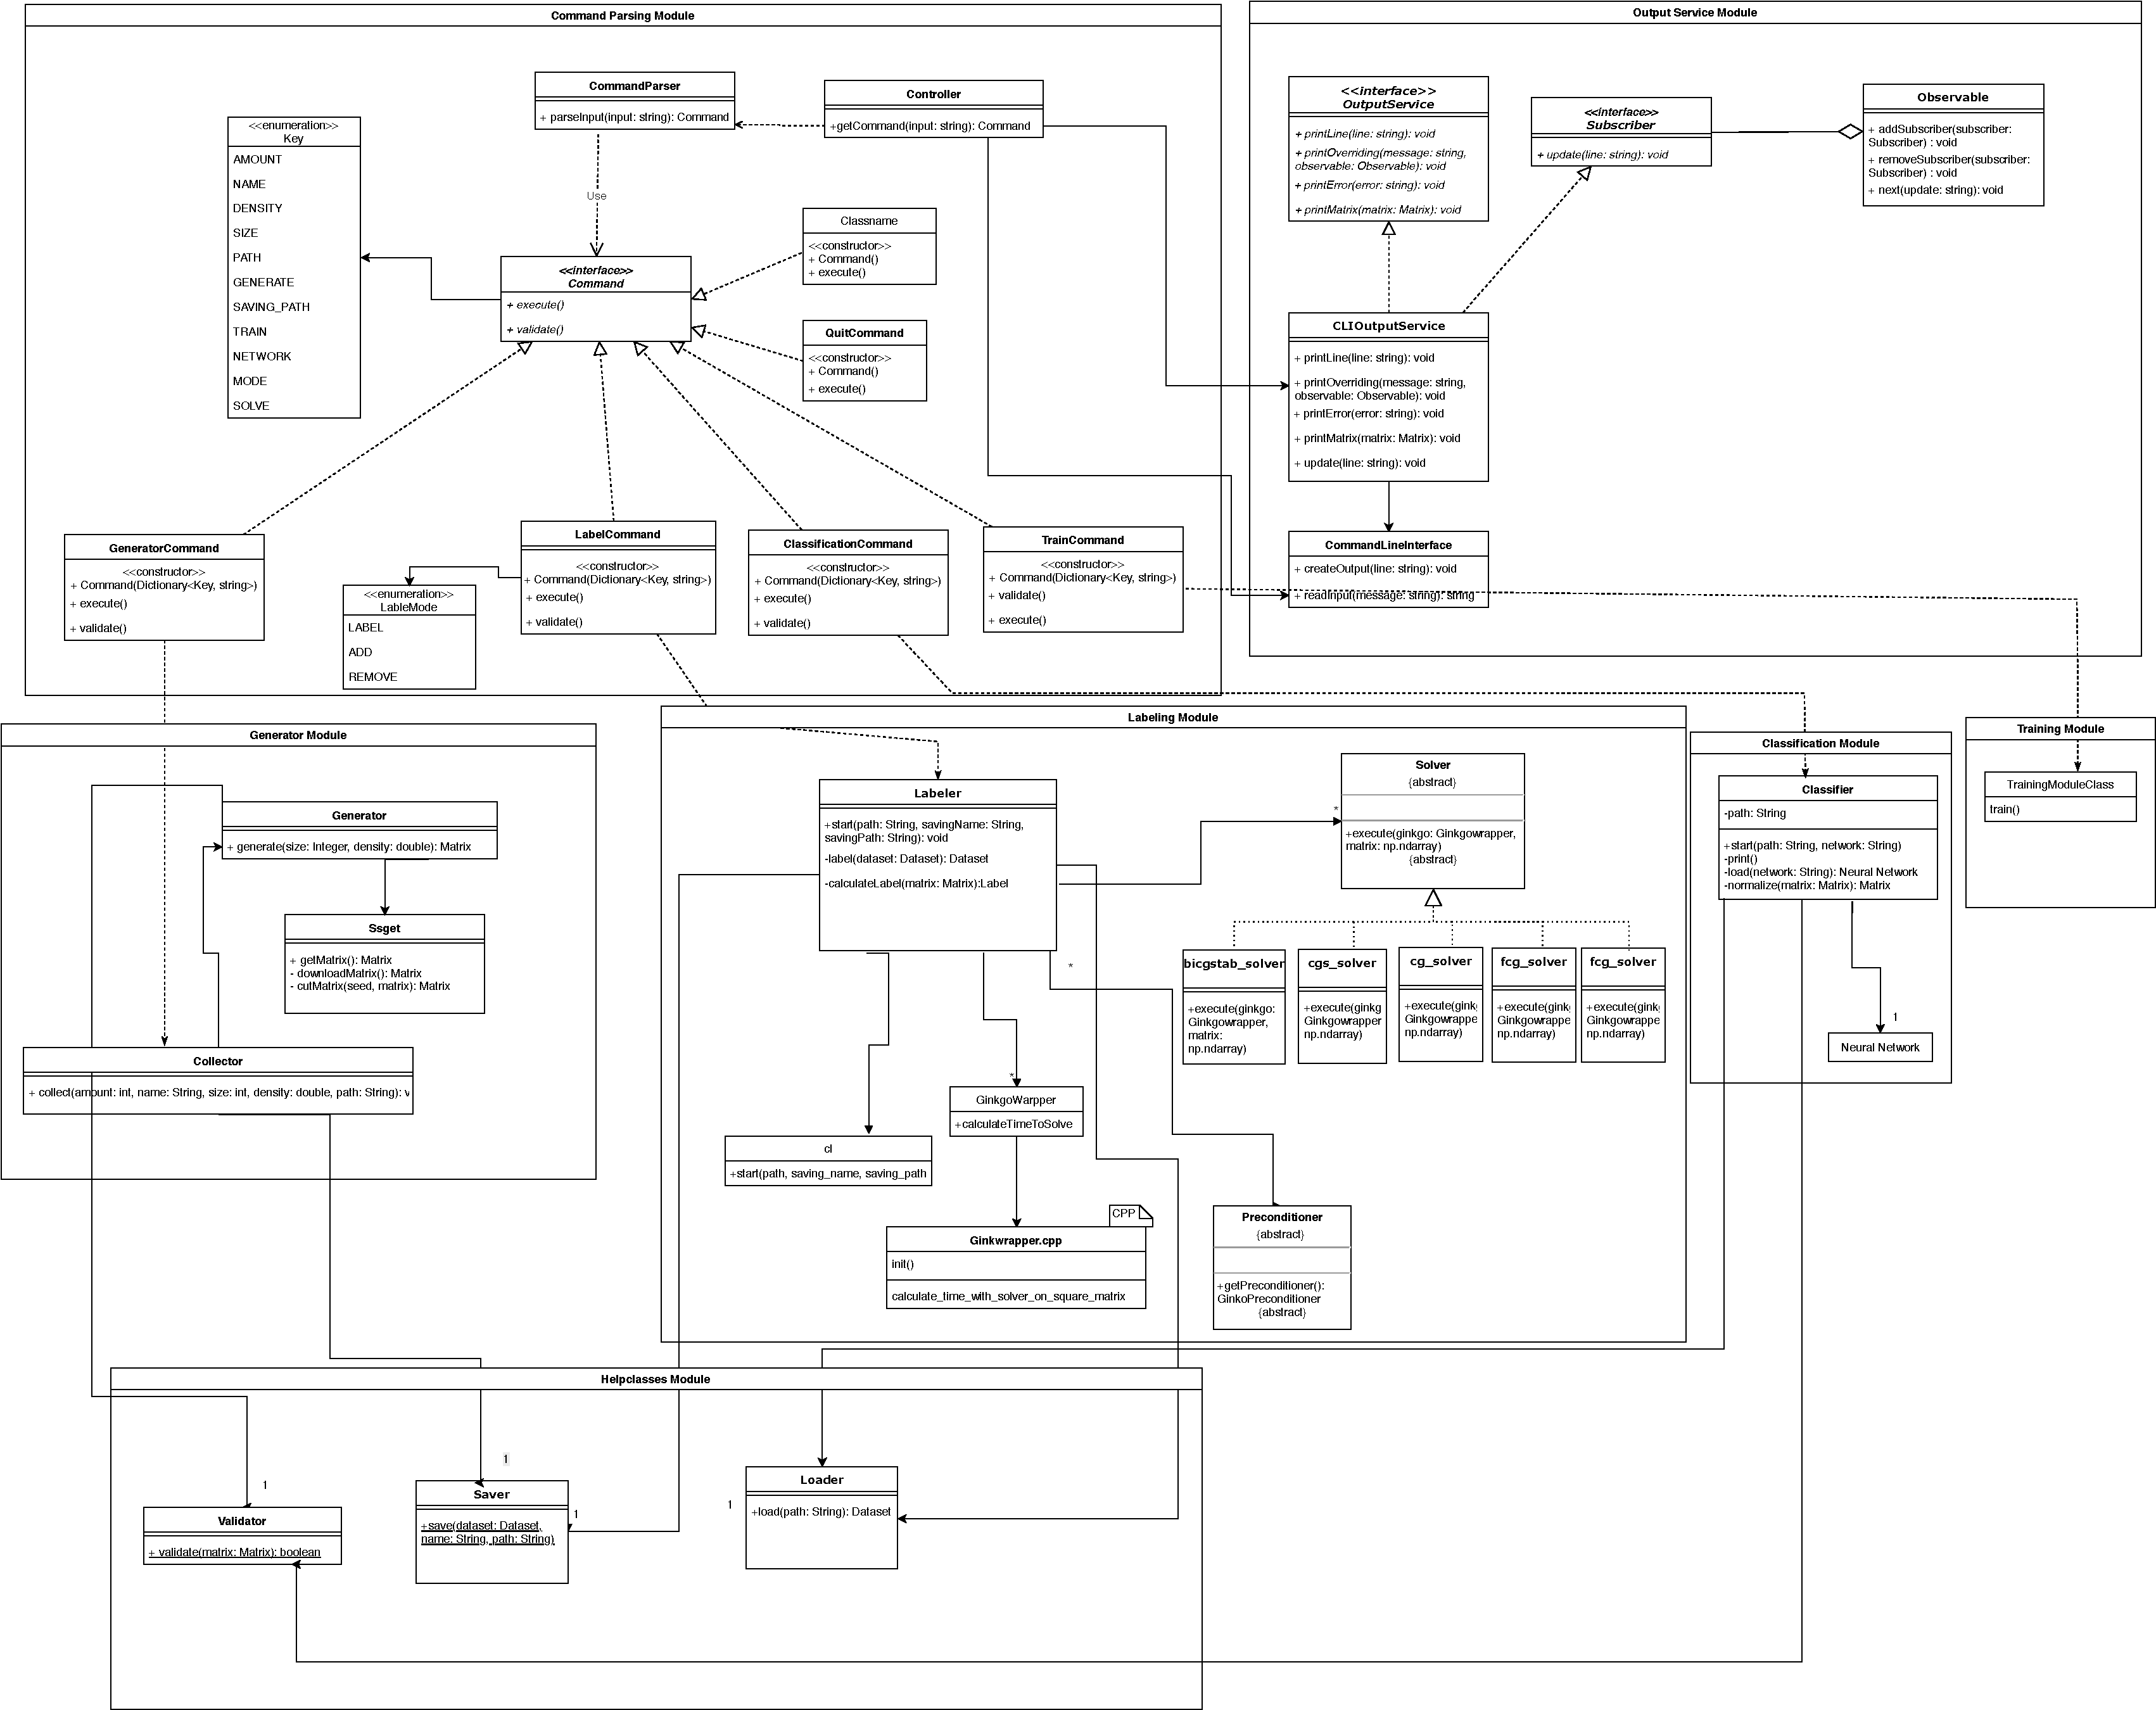
\includegraphics[width=\textwidth, height= \textheight, keepaspectratio]{../Big_classdiagram/Big_classdiagram.pdf}
    \caption{Big class diagram after design changes}
    \label{fig:PropProf}
\end{sidewaysfigure}


\newpage
\section{Glossary}
%\glspl{collector}, labeling modle, neural network, classifier, default settings  \glspl{Dateiformat}

% % Automatisch generiertes Glossar (Latex zwei mal ausführen um Glossar anzuzeigen)
%
%\glsaddall % das sorgt dafür, dass alles Glossareinträge gedruckt werden, nicht nur die verwendeten. Das sollte nicht nötig sein!
\printnoidxglossaries

\end{document}

